\documentclass[12pt, a4paper, oneside, openright, titlepage]{book}
\usepackage[utf8]{inputenc}
\raggedbottom
\usepackage{import}


%%%%%%%%%%%%%%%%% Book Formatting Comments:

%%%%%%%%%%%%%%%%%%%%%%%%%%%%%%%%%%%%% for Part

%%%%%%%%%%%%%%%%%%%%%% for chapter

%%%%%%%%%%%%%%%%%%%% for section




%%%%%% PACKAGES %%%%%%%
\usepackage{hyperref}
\hypersetup{
    colorlinks,
    citecolor=black,
    filecolor=black,
    linkcolor=black,
    urlcolor=black
}
\usepackage{amsmath} % Math display options
\usepackage{amssymb} % Math symbols
%\usepackage{amsfonts} % Math fonts
%\usepackage{amsthm}
\usepackage{mathtools} % General math tools
\usepackage{array} % Allows you to write arrays
\usepackage{empheq} % For boxing equations
% \usepackage{mathabx}
% \usepackage{mathrsfs}
\usepackage{nameref}
\usepackage{wrapfig}

\usepackage{soul}
\usepackage[normalem]{ulem}

\usepackage{txfonts}
\usepackage{cancel}
\usepackage[toc, page]{appendix}
\usepackage{titletoc,tocloft}
\setlength{\cftchapindent}{1em}
\setlength{\cftsecindent}{2em}
\setlength{\cftsubsecindent}{3em}
%\setlength{\cftsubsubsecindent}{4em}
\usepackage{titlesec}

%\titleformat{\section}
%  {\normalfont\fontsize{25}{15}\bfseries}{\thesection}%{1em}{}
%\titleformat{\section}
%  {\normalfont\fontsize{20}{15}\bfseries}%{\thesubsection}{1em}{}
%\setcounter{secnumdepth}{1}  
  
  

%\newcommand\numberthis{\refstepcounter{equation}\tag{\theequation}} % For equation labelling
\usepackage[framemethod=tikz]{mdframed}

\usepackage{tikz} % For drawing commutative diagrams
\usetikzlibrary{cd}
\usetikzlibrary{calc}
\tikzset{every picture/.style={line width=0.75pt}} %set default line width to 0.75p

\usepackage{datetime}
\usepackage[margin=1.5in]{geometry}
\setlength{\parskip}{1em}
\usepackage{makeidx}         % allows index generation
\usepackage{graphicx}       % standard LaTeX graphics tool
\usepackage{multicol}        % used for the two-column index
\usepackage[bottom]{footmisc}% places footnotes at page bottom

\usepackage{newtxtext}       % 
\usepackage{newtxmath}       % selects Times Roman as basic font
\usepackage{float}
\usepackage{fancyhdr}
\setlength{\headheight}{15pt} 
\pagestyle{fancy}
\lhead[\leftmark]{}
\rhead[]{\leftmark}

%\usepackage{enumitem}

\usepackage{url}
\allowdisplaybreaks

%%%%%% ENVIRONMENTS %%%
\definecolor{purp}{rgb}{0.29, 0, 0.51}
\definecolor{bloo}{rgb}{0, 0.13, 0.80}



%%\newtheoremstyle{note}% hnamei
%{3pt}% hSpace above
%{3pt}% hSpace belowi
%{}% hBody fonti
%{}% hIndent amounti
%{\itshape}% hTheorem head fonti
%{:}% hPunctuation after theorem headi
%{.5em}% hSpace after theorem headi
%{}% hTheorem head spec (can be left empty, meaning ‘normal’)i





% %%%%%%%%%%%%% THEOREM DEFINITIONS

\spnewtheorem{axiom}{Axiom}[chapter]{\bfseries}{\itshape}


\spnewtheorem{construction}{Construction}[chapter]{\bfseries}{\itshape}

\spnewtheorem{props}{Properties}[chapter]{\bfseries}{\itshape}


\renewcommand{\qedsymbol}{$\blacksquare$}


\numberwithin{equation}{section}

\newenvironment{qest}{
    \begin{center}
        \em
    }
    {
    \end{center}
    }

%%%%%% MACROS %%%%%%%%%
%% New Commands
\newcommand{\ip}[1]{\langle#1\rangle} %%% Inner product
\newcommand{\abs}[1]{\lvert#1\rvert} %%% Modulus
\newcommand\diag{\operatorname{diag}} %%% diag matrix
\newcommand\tr{\mbox{tr}\.} %%% trace
\newcommand\C{\mathbb C} %%% Complex numbers
\newcommand\R{\mathbb R} %%% Real numbers
\newcommand\Z{\mathbb Z} %%% Integers
\newcommand\Q{\mathbb Q} %%% Rationals
\newcommand\N{\mathbb N} %%% Naturals
\newcommand\F{\mathbb F} %%% An arbitrary field
\newcommand\ste{\operatorname{St}} %%% Steinberg Representation
\newcommand\GL{\mathbf{GL}} %%% General Linear group
\newcommand\SL{\mathbf{SL}} %%% Special linear group
\newcommand\gl{\mathfrak{gl}} %%% General linear algebra
\newcommand\G{\mathbf{G}} %%% connected reductive group
\newcommand\g{\mathfrak{g}} %%% Lie algebra of G
\newcommand\Hbf{\mathbf{H}} %%% Theta fixed points of G
\newcommand\X{\mathbf{X}} %%% Symmetric space X
\newcommand{\catname}[1]{\normalfont\textbf{#1}}
\newcommand{\Set}{\catname{Set}} %%% Category set
\newcommand{\Grp}{\catname{Grp}} %%% Category group
\newcommand{\Rmod}{\catname{R-Mod}} %%% Category r-modules
\newcommand{\Mon}{\catname{Mon}} %%% Category monoid
\newcommand{\Ring}{\catname{Ring}} %%% Category ring
\newcommand{\Topp}{\catname{Top}} %%% Category Topological spaces
\newcommand{\Vect}{\catname{Vect}_{k}} %%% category vector spaces'
\newcommand\Hom{\mathbf{Hom}} %%% Arrows

\newcommand{\map}[2]{\begin{array}{c} #1 \\ #2 \end{array}}

\newcommand{\Emph}[1]{\textbf{\ul{\emph{#1}}}}




%% Math operators
\DeclareMathOperator{\ran}{Im} %%% image
\DeclareMathOperator{\aut}{Aut} %%% Automorphisms
\DeclareMathOperator{\spn}{span} %%% span
\DeclareMathOperator{\ann}{Ann} %%% annihilator
\DeclareMathOperator{\rank}{rank} %%% Rank
\DeclareMathOperator{\ch}{char} %%% characteristic
\DeclareMathOperator{\ev}{\bf{ev}} %%% evaluation
\DeclareMathOperator{\sgn}{sign} %%% sign
\DeclareMathOperator{\id}{Id} %%% identity
\DeclareMathOperator{\supp}{Supp} %%% support
\DeclareMathOperator{\inn}{Inn} %%% Inner aut
\DeclareMathOperator{\en}{End} %%% Endomorphisms
\DeclareMathOperator{\sym}{Sym} %%% Group of symmetries


%% Diagram Environments
\iffalse
\begin{center}
    \begin{tikzpicture}[baseline= (a).base]
        \node[scale=1] (a) at (0,0){
          \begin{tikzcd}
           
          \end{tikzcd}
        };
    \end{tikzpicture}
\end{center}
\fi




\newdateformat{monthdayyeardate}{%
    \monthname[\THEMONTH]~\THEDAY, \THEYEAR}
%%%%%%%%%%%%%%%%%%%%%%%

%%% Specific Macros %%%


%%%%%% BEGIN %%%%%%%%%%


\begin{document}

%%%%%% TITLE PAGE %%%%%

\begin{titlepage}
    \centering
    \scshape
    \vspace*{\baselineskip}
    \rule{\textwidth}{1.6pt}\vspace*{-\baselineskip}\vspace*{2pt}
    \rule{\textwidth}{0.4pt}
    
    \vspace{0.75\baselineskip}
    
    {\LARGE Classical Geometry: A Complete Guide}
    
    \vspace{0.75\baselineskip}
    
    \rule{\textwidth}{0.4pt}\vspace*{-\baselineskip}\vspace{3.2pt}
    \rule{\textwidth}{1.6pt}
    
    \vspace{2\baselineskip}
    Classical Geometry \\
    \vspace*{3\baselineskip}
    \monthdayyeardate\today \\
    \vspace*{5.0\baselineskip}
    
    {\scshape\Large Elijah Thompson, \\ Physics and Math Honors\\}
    
    \vspace{1.0\baselineskip}
    \textit{Solo Pursuit of Learning}
    \vfill
    \enlargethispage{1in}
    \begin{figure}[b!]
    \makebox[\textwidth]{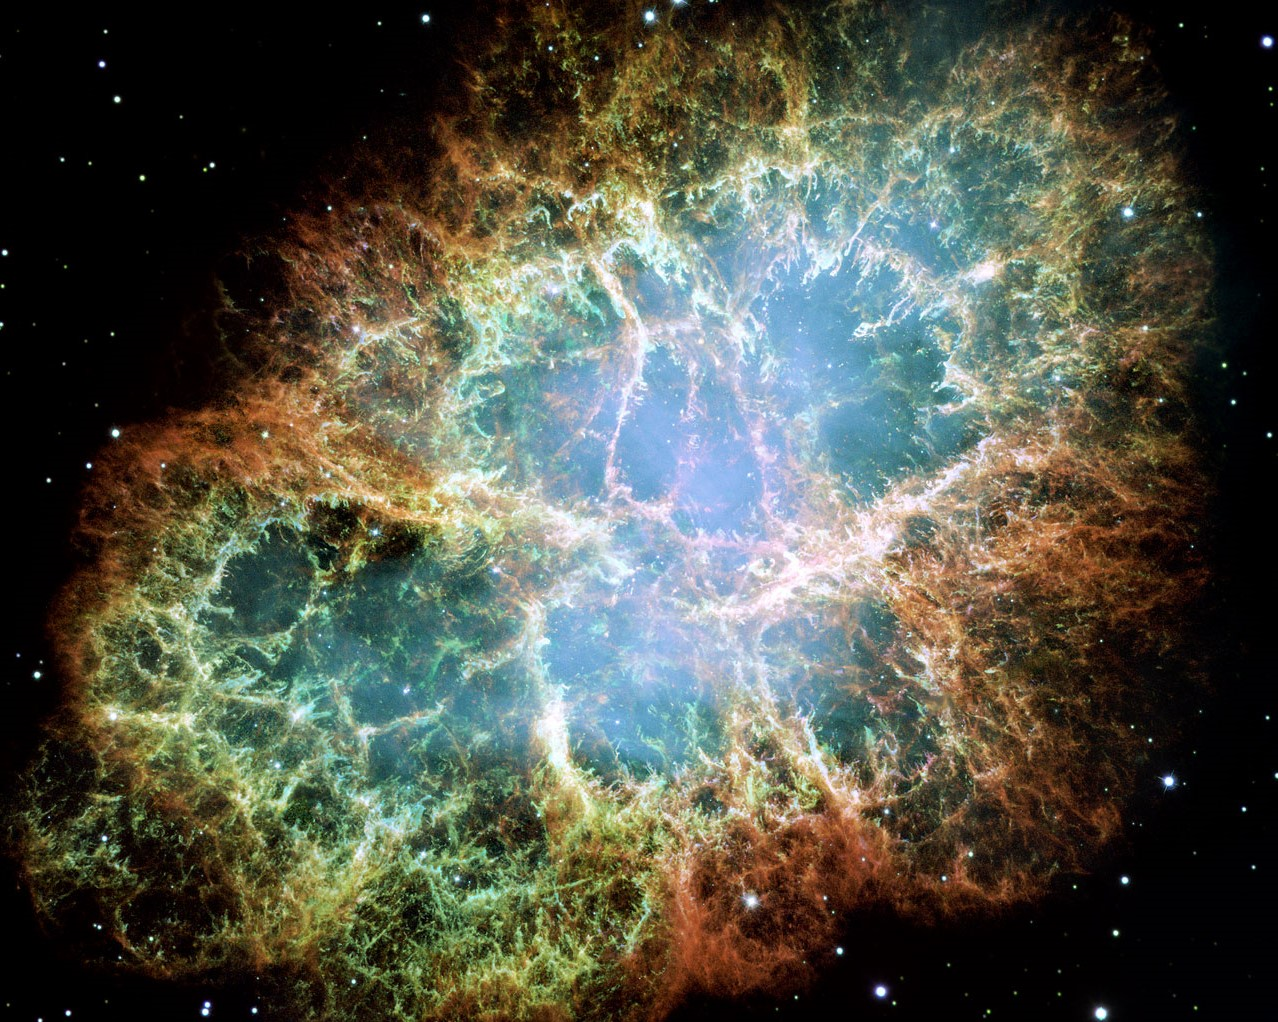
\includegraphics[width=\paperwidth, height =10cm]{../../Crab.jpg}}
    \end{figure}
\end{titlepage}

%%%%%%%%%%%%%%%%%%%%%%%
\tableofcontents


%%%%%%%%%%%%%%%%%%%%%%%%%%%%%%%%%%%% Part 1.
\part{Euclidean Geometry}

%%%%%%%%%%%%%%%%%%%%%% Chapter 1.1
\chapter{Length and the Dot Product}

We define the notion of a dot or scalar product of two vectors in euclidean n space as follows: 

\begin{defn}
    For vectors $u,v \in \R^n$ we define the \Emph{dot product} of $u$ and $v$ to be \begin{equation*}
        u\cdot v = \sum_{i=1}^nu_iv_i
    \end{equation*}
\end{defn}
Some important properties of the dot product, which show it is a positive definite, symmetric bilinear form on $\R^n$ are 

\begin{thm}[Properties of the Dot Product]
    For all $u,v,w \in \R^n$ and all $t \in \R$ we have \begin{enumerate}
        \item (Bilinearity) $(u+v)\cdot w = u\cdot w + v\cdot w, (tu)\cdot v = t(u\cdot v)$ and $u\cdot (v+w) = u\cdot v + u\cdot w, u \cdot (tv) = t(u\cdot v)$
        \item (Symmetry) $u\cdot v = v\cdot u$, and 
        \item (Positive Definiteness) $u\cdot u \geq 0$ with $u \cdot u = 0$ if and only if $u = 0$
    \end{enumerate}
\end{thm}

Using the dot product we can define a norm on $\R^n$:

\begin{defn}
    For a vector $u \in \R^n$, we define the \Emph{length} or \Emph{norm} of $u$ to be \begin{equation*}
        |u| = \sqrt{u\cdot u} = \sqrt{\sum_{i=1}^nu_i^2}
    \end{equation*}
\end{defn}

We say that $u$ is a \Emph{unit vector} when $|u| = 1$. From properties of the dot product we have the following properties of the norm:

\begin{thm}[Properties of the Length]
    Let $u,v \in \R^n$ and let $t \in \R$. Then \begin{enumerate}
        \item (Positive Definiteness) $|u| \geq 0$ with $|u| = 0$ if and only if $u = 0$
        \item (Scaling) $|tu| = |t||u|$
        \item $|u\pm v|^2 = |u|^2\pm 2(u\cdot v)+|v|^2$ 
        \item (The Polarization Identities) $u\cdot v = \frac{1}{2}(|u+v|^2-|u|^2-|v|^2) = \frac{1}{4}(|u+v|^2-|u-v|^2)$
        \item (The Cauchy-Schwarz Inequality) $|u\cdot v| \leq |u||v|$ with $|u\cdot v| = |u||v|$ if and only if the set $\{u,v\}$ is linearly dependent,
        \item (The Triangle Inequality) $|u+v| \leq |u|+|v|$
    \end{enumerate}
\end{thm}

Next, we can use the norm to define a metric, or distance, for $\R^n$:

\begin{defn}
    For points $u,v \in \R^n$, we define the Euclidean \Emph{distance} between $u$ and $v$ to be \begin{equation*}
        d_E(u,v) := |v-u|
    \end{equation*}
\end{defn}

The following theorem proves that this distance is indeed a metric:

\begin{thm}[Metric Properties of the Euclidean Distance]
    Let $u,v,w \in \R^n$. Then \begin{enumerate}
        \item (Positive Definiteness) $d_E(u,v) \geq 0$ with $d_E(u,v) = 0$ if and only if $u = v$,
        \item (Symmetry) $d_E(u,v) = d_E(v,u)$ 
        \item (The Triangle Inequality) $d_E(u,w) \leq d_E(u,v) + d_E(v,w)$
    \end{enumerate}
\end{thm}




%%%%%%%%%%%%%%%%%%%% Section 1.1.1



%%%%%%%%%%%%%%%%%%%%%% - Appendices
\begin{appendices}


\end{appendices}


\end{document}


%%%%%% END %%%%%%%%%%%%%
